% !TEX encoding = UTF-8 Unicode

\chapter{Die \boldmath{$\alpha$}-Shape}

Die $\alpha$-Shape wird mit Kreisscheiben mit einem Radius vom Betrag $\alpha$ bestimmt. Diese Kreisscheiben werden auch zur Konstruktion der $\alpha$-Hülle verwendet werden. Hier wird nun zuerst auf die $\alpha$-Hülle eingegangen und im Folgenden die $\alpha$-Shape definiert.

In \autocite{alpha1983} ist $\alpha$ der Kehrwert des Radius einer Kreisscheibe und es werden auch Komplemente dieser Kreisscheiben verwendet. In dieser Darstellung wurde auf die Verwendung der Komplemente von Kreisscheiben verzichtet.

Für die folgenden Definitionen sei eine Punktmenge $S$ gegeben. Die definierten Begriffe beziehen sich immer auf diese Punktmenge.

\section[Die $\alpha$-Hülle]{Die \boldmath{$\alpha$}-Hülle}

Die $\alpha$-Hülle ist abhängig von einem Parameter $\alpha$. Der Parameter $\alpha$ bestimmt dabei den Radius derjenigen Kreisscheiben, welche zu ihrer Konstruktion verwendet werden. Je nachdem ob $\alpha$ positiv oder negativ ist, wird die $\alpha$-Hülle unterschiedlich definiert. Für die verwendeten Kreisscheiben wird hier der Begriff der $\alpha$-Kreisscheibe eingeführt.

\begin{defin}
Für $\alpha > 0$ ist eine offene Kreisscheibe mit Radius $\alpha$ eine \emph{$\alpha$-Kreisscheibe}, genau dann wenn diese keinen Punkt aus $S$ enthält. Eine solche Kreisscheibe wird auch \emph{positive $\alpha$-Kreisscheibe} genannt.\\
Für $\alpha < 0$ ist eine abgeschlossene Kreisscheibe mit einem Radius vom Betrag $\alpha$ eine \emph{$\alpha$-Kreisscheibe}, genau dann wenn diese alle Punkte aus $S$ enthält. Eine solche Kreisscheibe wird auch \emph{negative $\alpha$-Kreisscheibe} genannt.
\end{defin}

\begin{figure}[htbp]
	\centering
	\subfloat[Positive $\alpha$-Kreisscheibe\label{fig:alphaDisc_positive}]
		{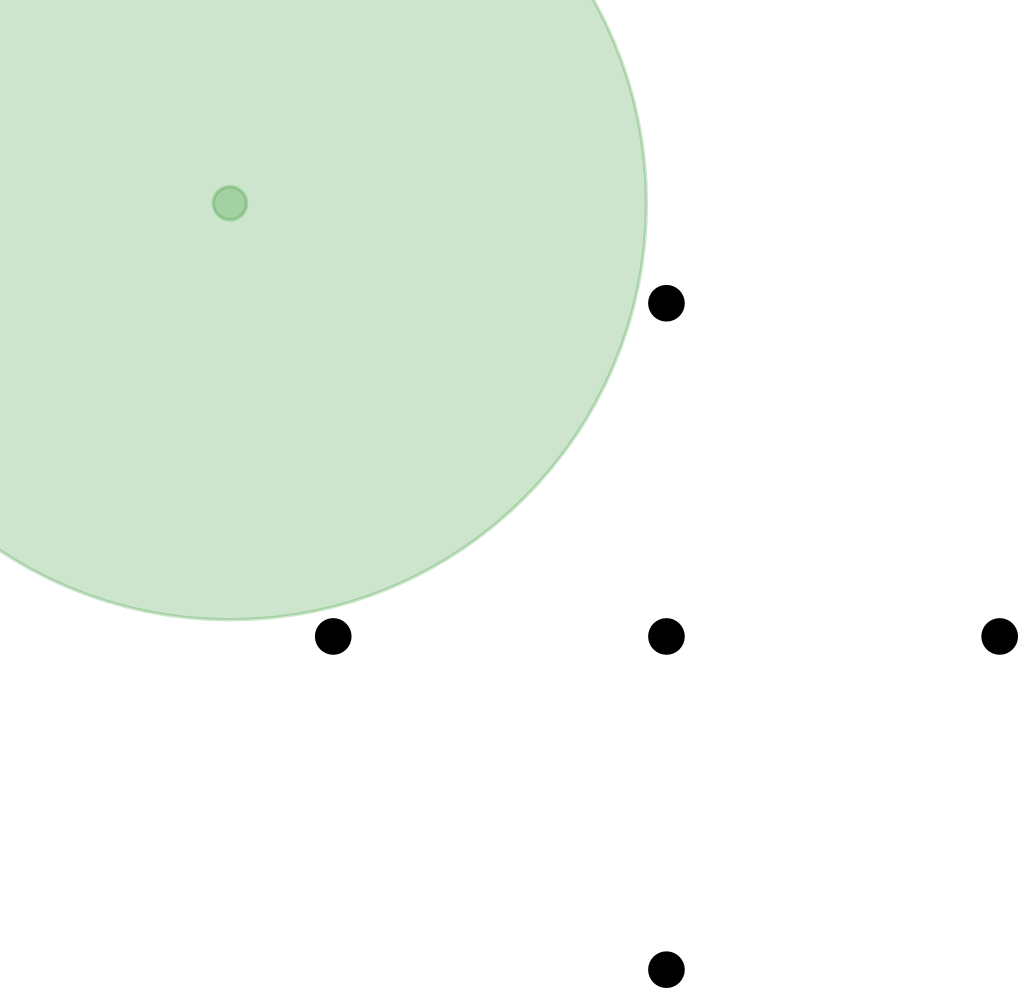
\includegraphics[scale=0.7]{../bilder/alphaDisc_positive.png}}
	\hspace{2cm}
	\subfloat[Negative $\alpha$-Kreisscheibe\label{fig:alphaDisc_negative}]
		{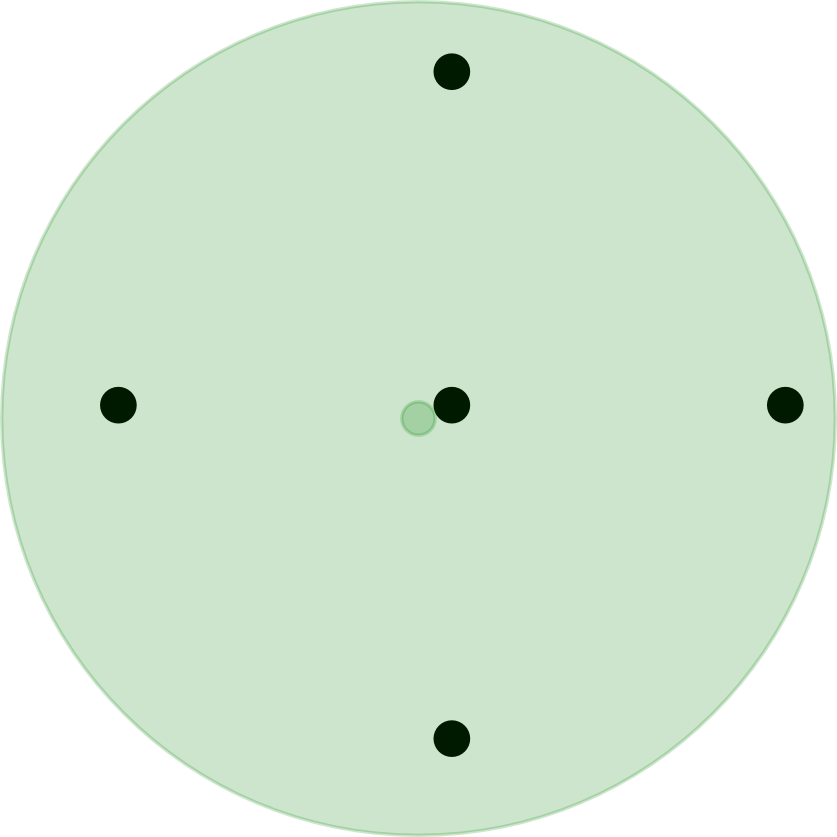
\includegraphics[scale=0.7]{../bilder/alphaDisc_negative.png}}
	\caption{$\alpha$-Kreisscheiben}
	\label{fig:alphaDiscs}	
\end{figure}

In Abbildung~\ref{fig:alphaDiscs} sind $\alpha$-Kreisscheiben mit betragsmäßig gleichem Radius dargestellt. Abbildung~\ref{fig:alphaDisc_positive} stellt eine positive $\alpha$-Kreisscheibe dar und Abbildung~\ref{fig:alphaDisc_negative} eine negative.

Mit Hilfe der $\alpha$-Kreisscheiben wird nun die $\alpha$-Hülle definiert.

\begin{defin}
Für $\alpha > 0$ ist die \emph{$\alpha$-Hülle} gleich dem Komplement der Vereinigung aller $\alpha$-Kreisscheiben. Diese $\alpha$-Hülle wird auch \emph{positive $\alpha$-Hülle} genannt.\\
Für $\alpha < 0$ ist die $\alpha$-Hülle gleich der Schnittfläche aller $\alpha$-Kreisscheiben. Diese $\alpha$-Hülle wird auch \emph{negative $\alpha$-Hülle} genannt.
\end{defin}

Existieren für ein $\alpha < 0$ keine $\alpha$-Kreisscheiben, so ist die $\alpha$-Hülle gleich der Ebene.

\begin{figure}[htbp]
	\centering
	\subfloat[Positive $\alpha$-Hülle\label{fig:alphaHull_positive}]
		{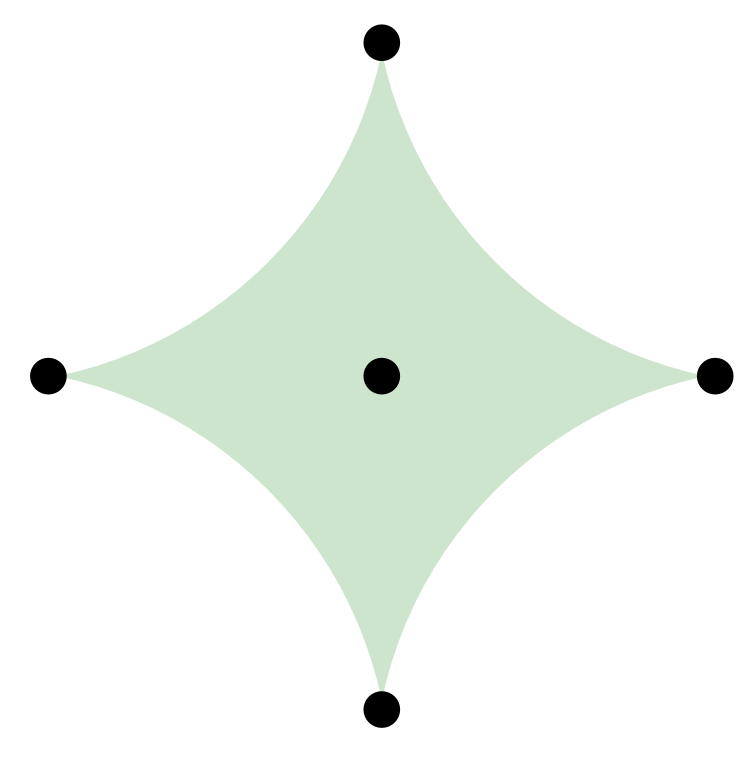
\includegraphics[scale=0.7]{../bilder/alphaHull_positive.png}}
	\hspace{2cm}
	\subfloat[Negative $\alpha$-Hülle\label{fig:alphaHull_negative}]
		{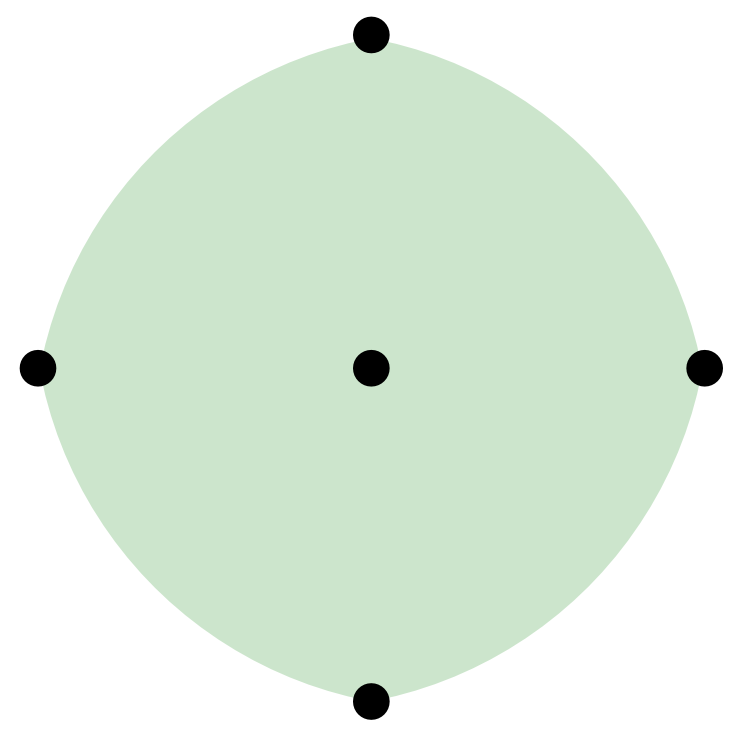
\includegraphics[scale=0.7]{../bilder/alphaHull_negative.png}}
	\caption{$\alpha$-Hüllen}
	\label{fig:alphaHulls}	
\end{figure}

In Abbildung~\ref{fig:alphaHulls} sind positive und negative $\alpha$-Hüllen dargestellt. Der Radius der $\alpha$-Kreisscheiben ist gleich derer in Abbildung~\ref{fig:alphaDiscs}.

Die $\alpha$-Hülle kann auch als Verallgemeinerung der konvexen Hülle betrachtet werden. Für betragsmäßig unendlich große $\alpha$ werden die $\alpha$-Kreisscheiben zu Halbebenen. Dann ist die $\alpha$-Hülle gleich der konvexen Hülle.

\begin{defin}
Die \emph{konvexe Hülle} ist die Schnittfläche aller abgeschlossenen Halbebenen, welche alle Punkte aus $S$ beinhalten.\\
Alternativ kann die konvexe Hülle auch als Komplement zur Vereinigung aller offenen Halbebenen, welche keinen Punkt aus $S$ beinhalten, betrachtet werden.
\end{defin}

\begin{figure}[htbp]
	\centering
	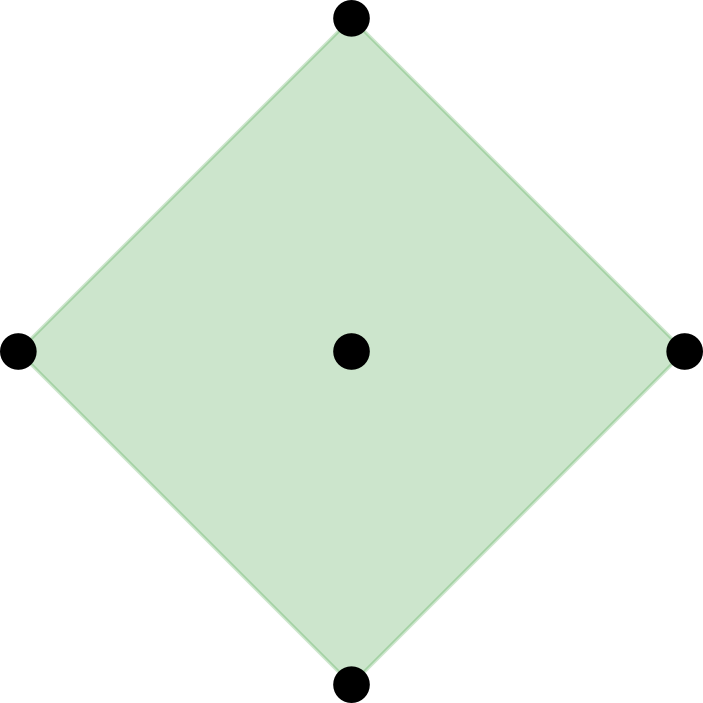
\includegraphics[scale=0.7]{../bilder/convexHull.png}
	\caption{Konvexe Hülle}
	\label{fig:convexHull}	
\end{figure}

In Abbildung~\ref{fig:convexHull} ist die konvexe Hülle der in Abbildung~\ref{fig:alphaDiscs} und \ref{fig:alphaHulls} verwendeten Punktmenge dargestellt.

\section[Die $\alpha$-Shape]{Die \boldmath{$\alpha$}-Shape}

Die $\alpha$-Shape ist ein Graph, dessen Knotenmenge eine Teilmenge von $S$ ist. Knoten der $\alpha$-Shape werden $\alpha$-extreme Punkte genannt.

\begin{defin}
Ein Punkt aus $S$ ist \emph{$\alpha$-extrem}, genau dann wenn er auf dem Rand einer $\alpha$-Kreisscheibe liegt.
\end{defin}

\begin{figure}[htbp]
	\centering
	\subfloat[$\alpha$-extremer Punkt auf positiver $\alpha$-Kreisscheibe\label{fig:alphaExtreme_positive}]
		{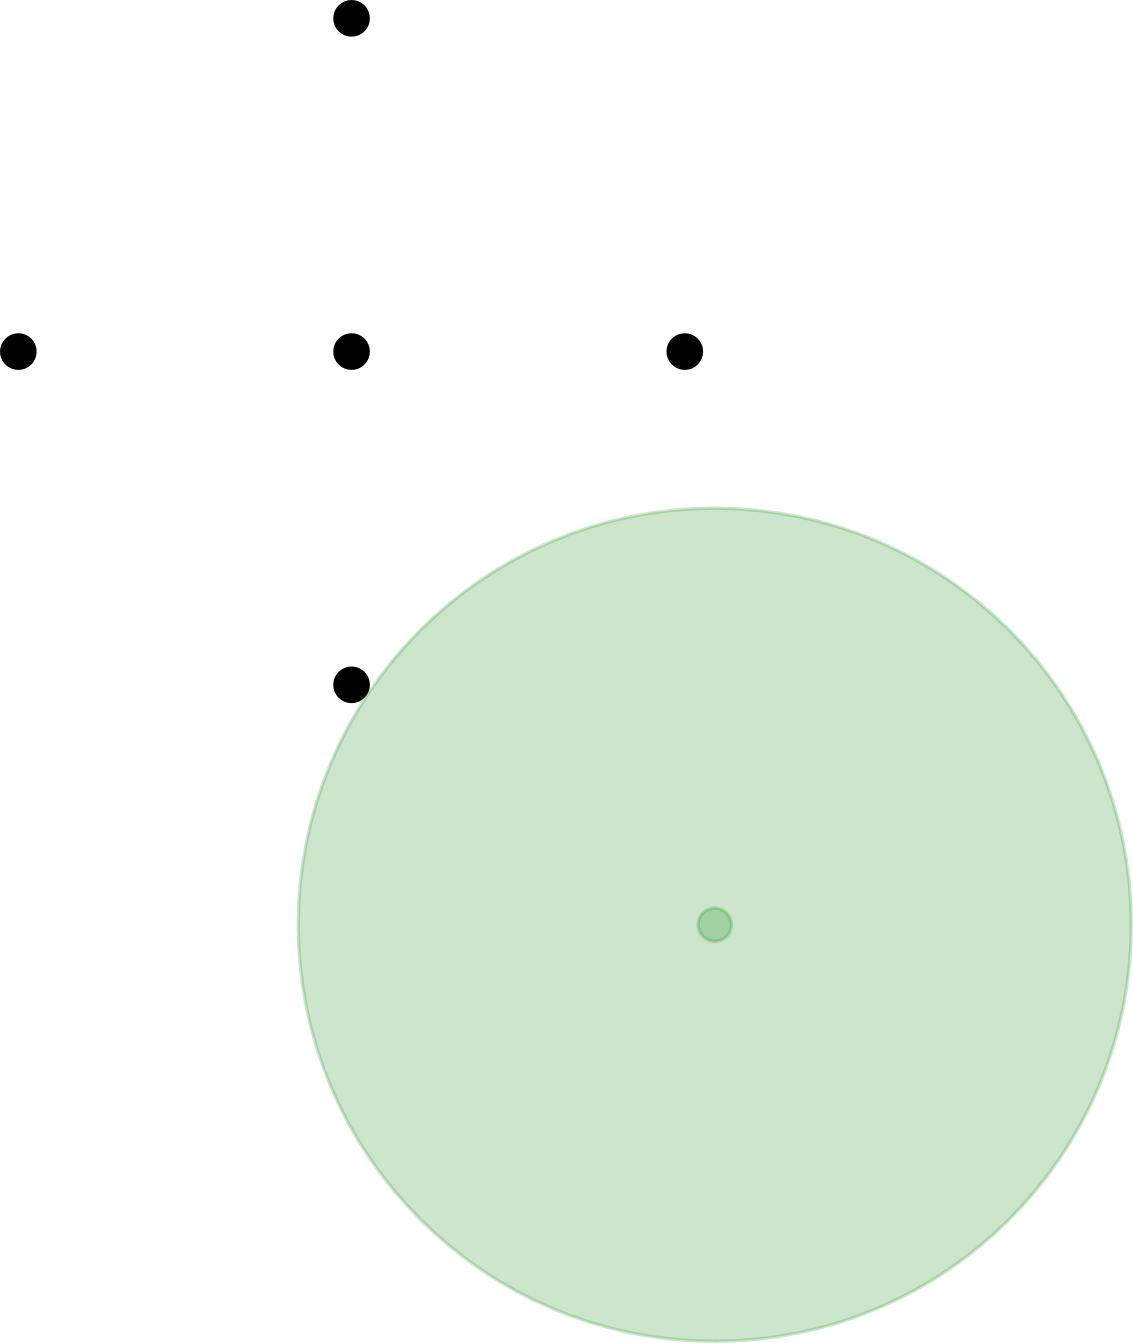
\includegraphics[scale=0.7]{../bilder/alphaExtreme_positive.png}}
	\hspace{2cm}
	\subfloat[$\alpha$-extremer Punkt auf negativer $\alpha$-Kreisscheibe\label{fig:alphaExtreme_negative}]
		{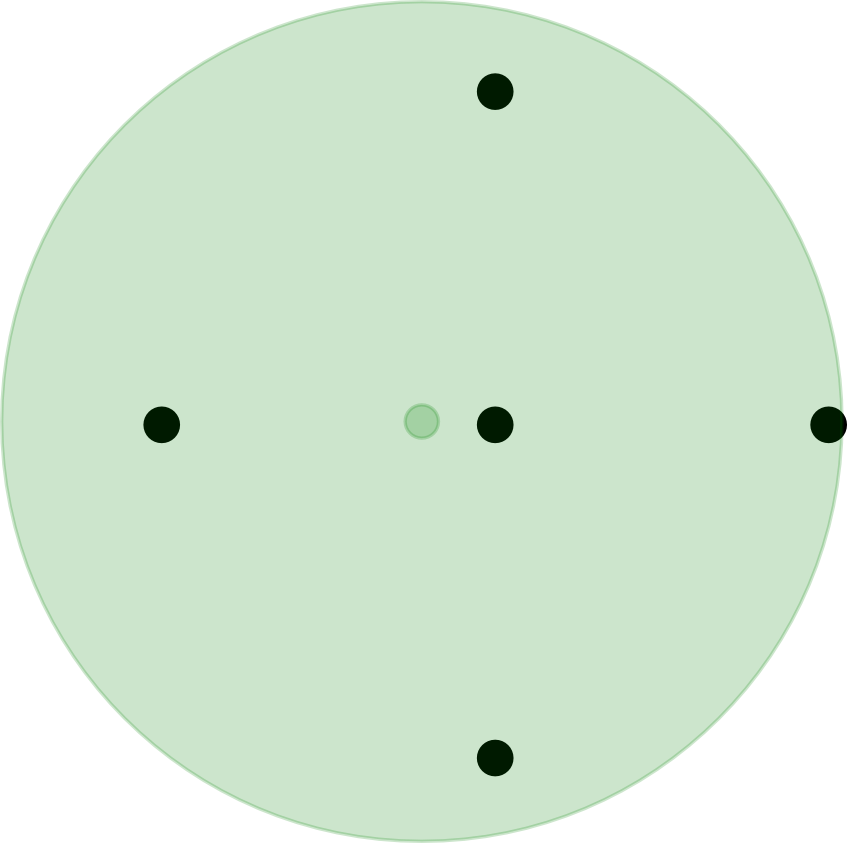
\includegraphics[scale=0.7]{../bilder/alphaExtreme_negative.png}}
	\caption{$\alpha$-extreme Punkte}
	\label{fig:alphaExtremes}	
\end{figure}

Abbildung~\ref{fig:alphaExtremes} zeigt $\alpha$-extreme Punkte auf dem Rand von positiven und negativen $\alpha$-Kreisscheiben.

\begin{defin}
Zwei Punkte aus $S$ sind \emph{$\alpha$-Nachbarn}, genau dann wenn sie auf dem Rand derselben $\alpha$-Kreisscheibe liegen und auf dieser direkt benachbart sind.
\end{defin}

\begin{figure}[htbp]
	\centering
	\subfloat[$\alpha$-Nachbarn auf positiver $\alpha$-Kreisscheibe\label{fig:alphaNeighbours_positive}]
		{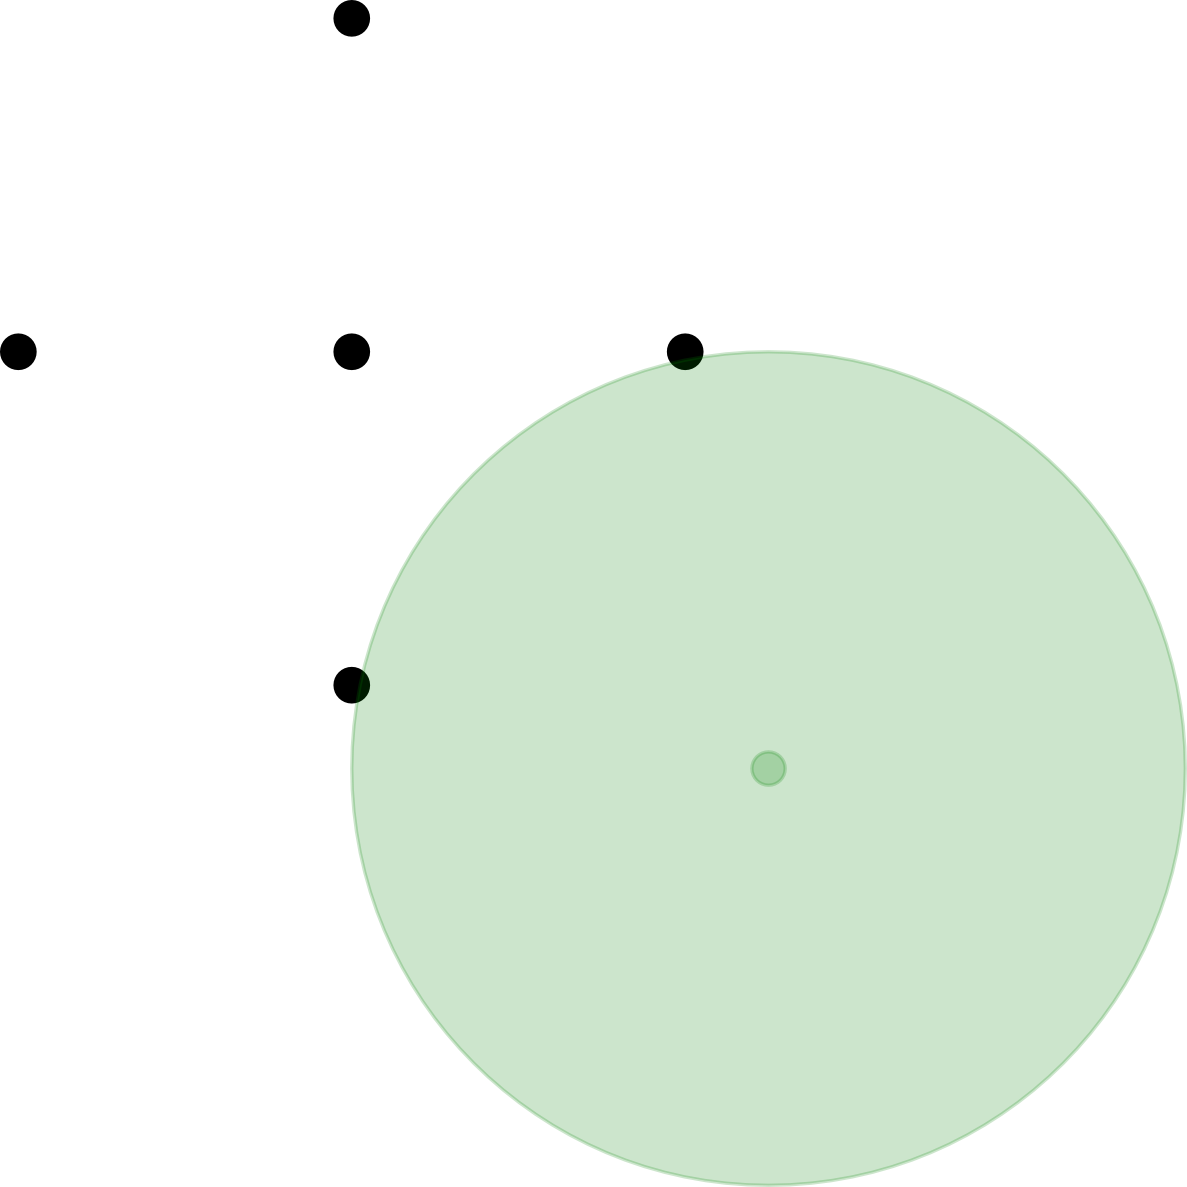
\includegraphics[scale=0.7]{../bilder/alphaNeighbours_positive.png}}
	\hspace{2cm}
	\subfloat[$\alpha$-Nachbarn auf negativer $\alpha$-Kreisscheibe\label{fig:alphaNeighbours_negative}]
		{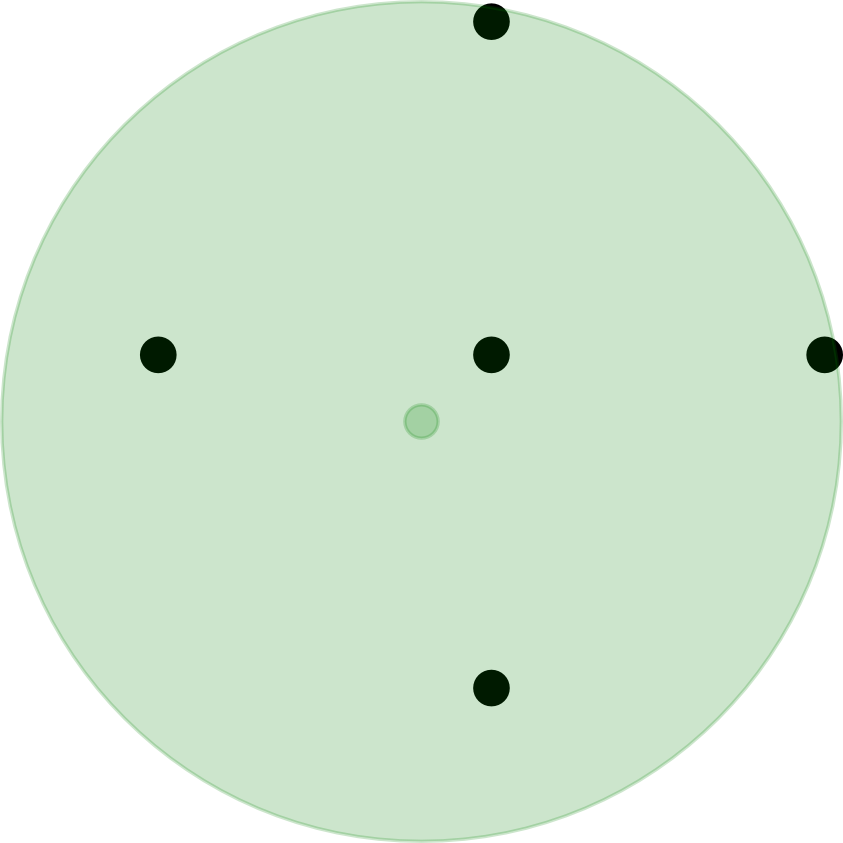
\includegraphics[scale=0.7]{../bilder/alphaNeighbours_negative.png}}
	\caption{$\alpha$-Nachbarn}
	\label{fig:alphaNeighbours}	
\end{figure}

Abbildung~\ref{fig:alphaNeighbours} zeigt $\alpha$-Nachbarn, welche jeweils auf einer positiven und einer negativen $\alpha$-Kreisscheibe liegen.

Mit Hilfe $\alpha$-extremer Punkte und $\alpha$-Nachbarn wird die $\alpha$-Shape folgendermaßen definiert.

\begin{defin}
Die \emph{$\alpha$-Shape} ist der Graph mit $\alpha$-extremen Punkten als Knoten und Kanten zwischen den $\alpha$-Nachbarn. Für ein $\alpha > 0$ wird die $\alpha$-Shape auch \emph{positive $\alpha$-Shape} genannt. Für ein $\alpha < 0$ wird die $\alpha$-Shape auch \emph{negative $\alpha$-Shape} genannt.
\end{defin}

\begin{figure}[htbp]
	\centering
	\subfloat[Positive $\alpha$-Shape\label{fig:alphaShape_positive}]
		{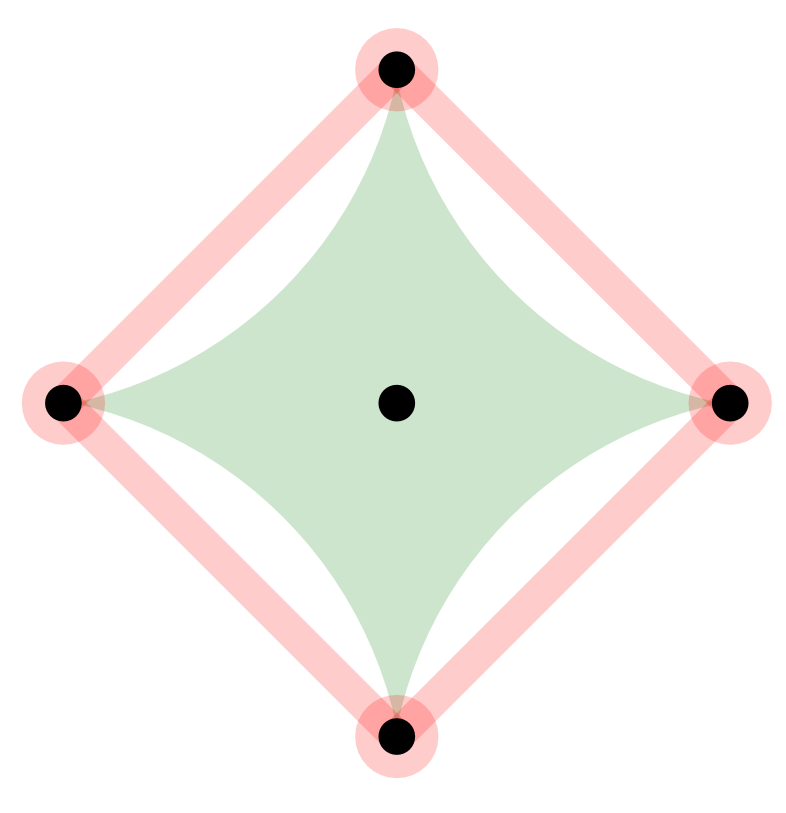
\includegraphics[scale=0.7]{../bilder/alphaShape_positive.png}}
	\hspace{2cm}
	\subfloat[Negative $\alpha$-Shape\label{fig:alphaShape_negative}]
		{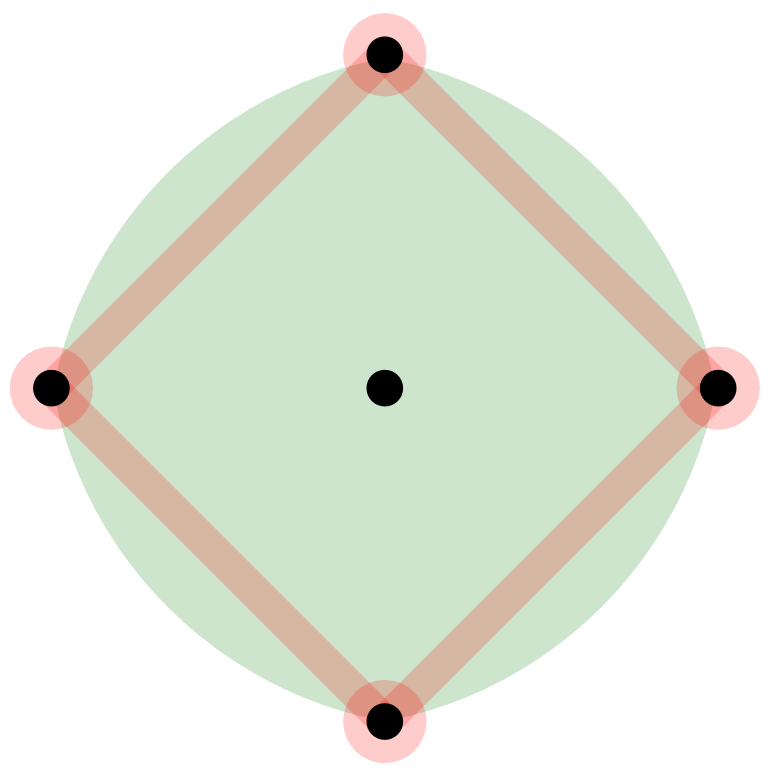
\includegraphics[scale=0.7]{../bilder/alphaShape_negative.png}}
	\caption{$\alpha$-Shapes}
	\label{fig:alphaShapes}	
\end{figure}

In Abbildung~\ref{fig:alphaShapes} sind positive und negative $\alpha$-Shapes und -Hüllen abgebildet.

Dadurch, dass nur Punkte, welche direkt auf einer $\alpha$-Kreisscheibe benachbart sind auch $\alpha$-Nachbarn sind, kreuzen sich Kanten der $\alpha$-Shape nicht.

\section[$\alpha$-Hüllen und -Shapes für verschiedene $\alpha$]{\boldmath{$\alpha$}-Hüllen und -Shapes für verschiedene \boldmath{$\alpha$}}

Für die folgenden Beispiele wird der Parameter $\alpha$ von betragsmäßig unendlich großen, negativen hin zu unendlich großen, positiven Werten variiert.

Für betragsmäßig unendlich große, negative Werte von $\alpha$ ist die $\alpha$-Hülle gleich der konvexen Hülle. Die $\alpha$-Shape liegt in diesem Fall auf dem Rand der konvexen Hülle.

\begin{figure}[htbp]
	\centering
	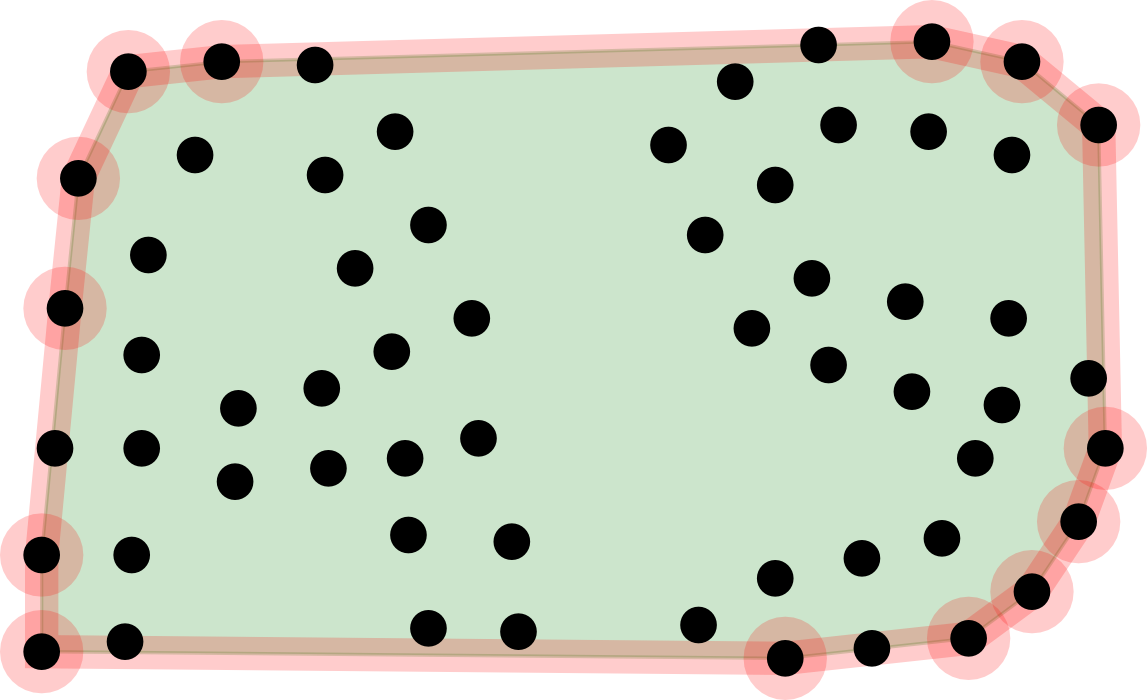
\includegraphics[scale=0.7]{../bilder/smallAS_shapeHull_convex.png}
	\caption{$\alpha$-Hülle gleich der konvexen Hülle}
	\label{fig:shapeHull_convex}
\end{figure}

Abbildung~\ref{fig:shapeHull_convex} stellt $\alpha$-Hülle und -Shape für den Fall dar, dass die $\alpha$-Hülle gleich der konvexen Hülle ist.

Bewegt sich $\alpha$ von betragsmäßig sehr großen, negativen Werten hin zu betragsmäßig kleineren, negativen Werten, so dehnt sich die $\alpha$-Hülle aus. Punkte aus $S$, welche für betragsmäßig größere $\alpha$ noch auf dem Rand der $\alpha$-Hülle gelegen sind, befinden sich nun im inneren der $\alpha$-Hülle. Diese Punkte sind somit nicht mehr $\alpha$-extrem und tragen nicht mehr zu $\alpha$-Shape bei.

\begin{figure}[htbp]
	\centering
	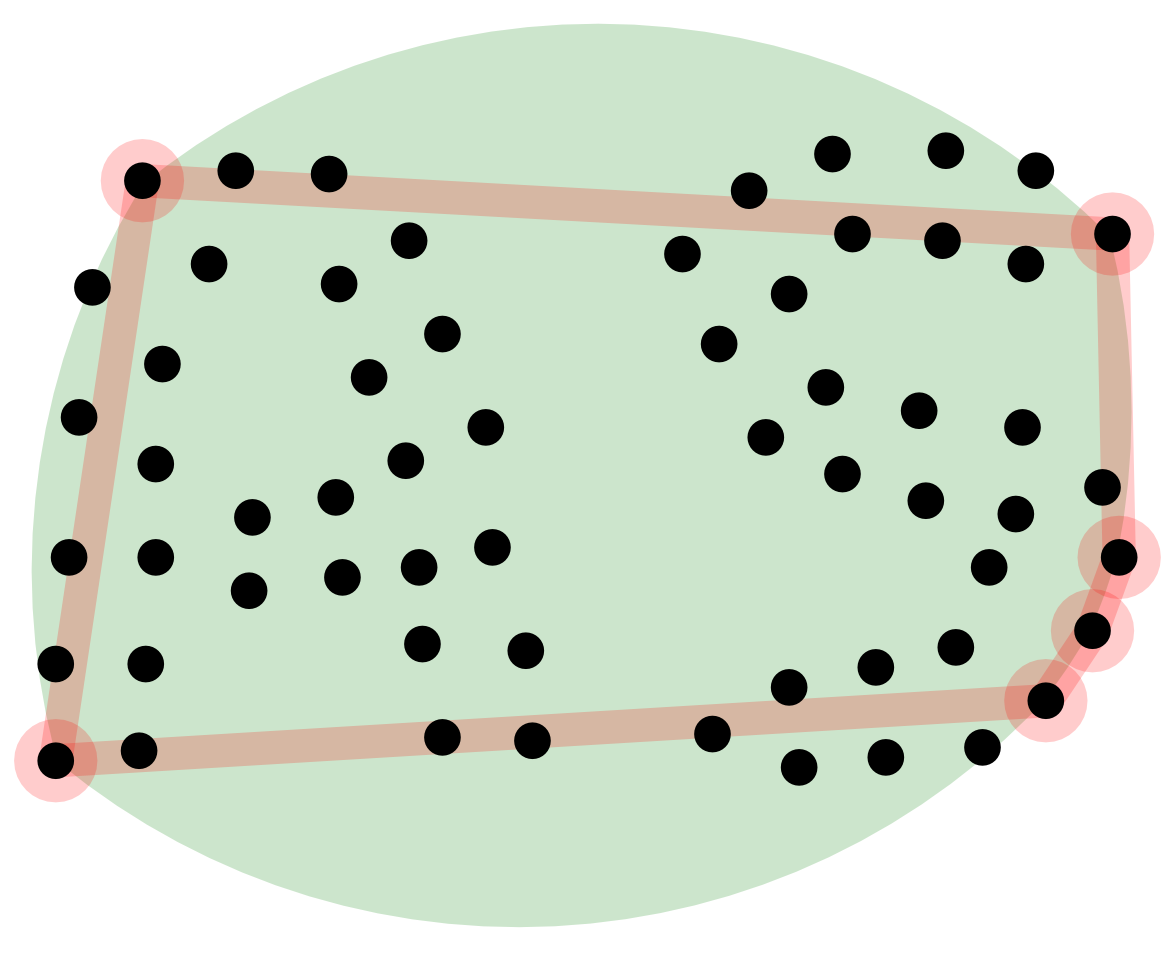
\includegraphics[scale=0.7]{../bilder/smallAS_shapeHull_negative.png}
	\caption{$\alpha$-Hülle und -Shape für negatives $\alpha$}
	\label{fig:shapeHull_negative}
\end{figure}

Abbildung~\ref{fig:shapeHull_negative} stellt den gerade geschilderten Fall einer $\alpha$-Shape und einer $\alpha$-Hülle dar.

Nun sei $\alpha$ gleich der Negation des Radius des kleinsten einschließenden Kreises der Punktmenge. In diesem Fall entspricht die $\alpha$-Hülle gleich der kleinsten negativen $\alpha$-Kreisscheibe. Diese Kreisscheibe wird von dem kleinsten einschließenden Kreis umrandet. Die Knotenmenge der $\alpha$-Shape ist die Menge derjenigen Punkte aus $S$, welche auf diesem Kreis liegen. Die Kanten der $\alpha$-Shape verbinden diejenigen Knoten, welche auf dem Kreis direkt benachbart sind.

\begin{figure}[htbp]
	\centering
	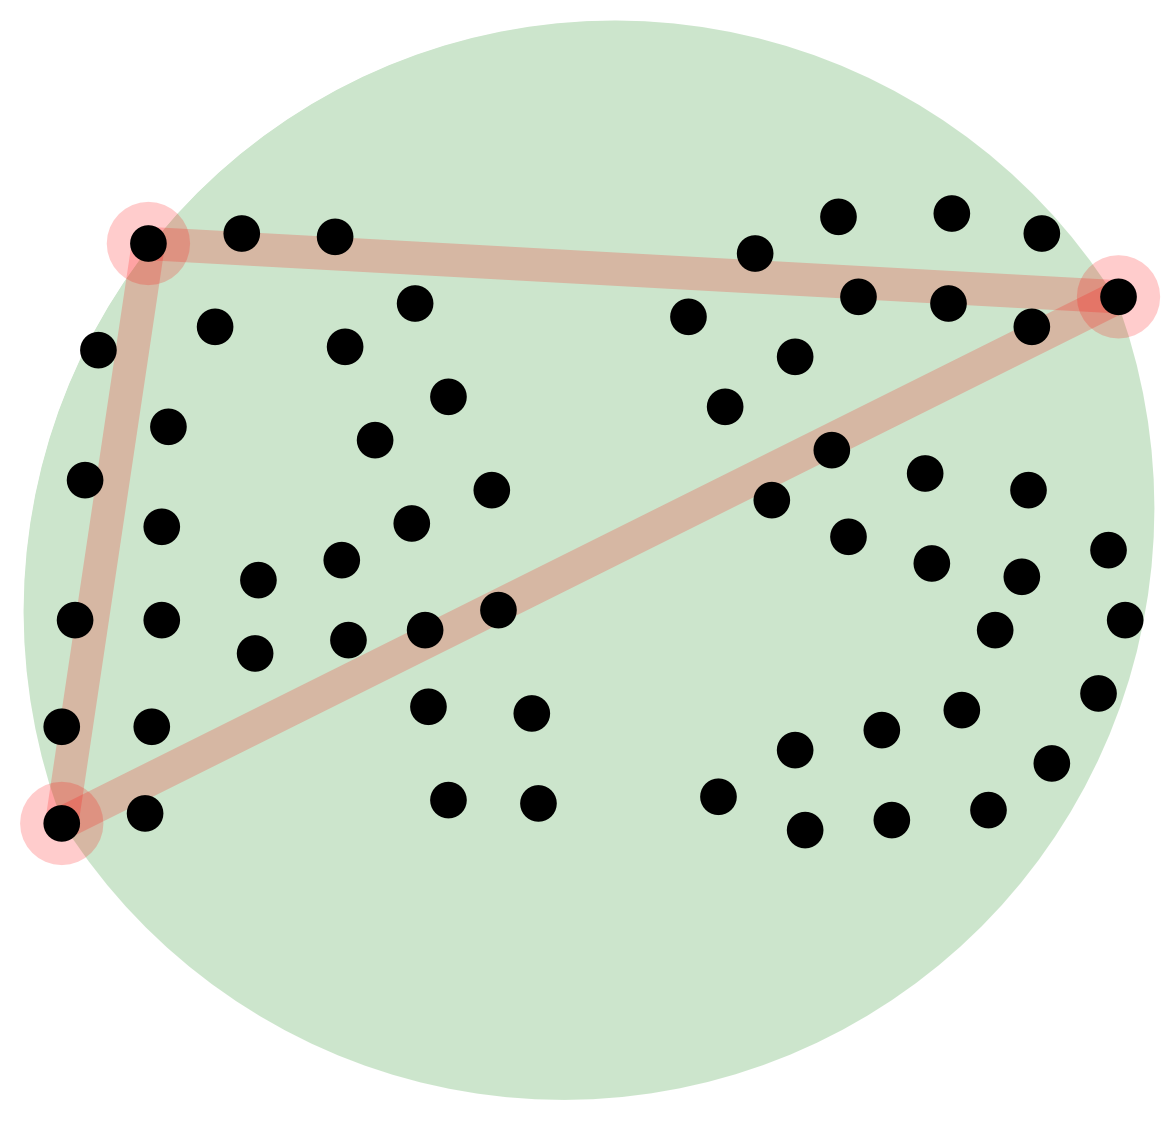
\includegraphics[scale=0.7]{../bilder/smallAS_shapeHull_smallestCircle.png}
	\caption{$\alpha$-Hülle gleich kleinster negativer $\alpha$-Kreisscheibe}
	\label{fig:shapeHull_smallestCircle}
\end{figure}

Abbildung~\ref{fig:shapeHull_smallestCircle} stellt einen Fall dar, indem drei Punkte auf der kleinsten möglichen negativen $\alpha$-Kreisscheibe liegen. Dies sind die $\alpha$-extremen Punkte, von denen jedes Paar auch $\alpha$-Nachbarn sind.

Für negative $\alpha$, welche vom Betrag her kleiner sind als der Radius des kleinsten einschließenden Kreises, existiert keine $\alpha$-Kreisscheibe mehr. Die $\alpha$-Hülle besteht nunmehr aus der gesamten Ebene. Die $\alpha$-Shape enthält keine Knoten und keine Kanten, da keine $\alpha$-extremen Punkte und somit auch keine $\alpha$-Nachbarn existieren.

Für ein $\alpha = 0$ sind $\alpha$-Hülle und -Shape nicht definiert.

Ist ein positives $\alpha$ kleiner als die Hälfte des Abstands des dichtesten Paares, so ist die $\alpha$-Hülle leer. Die Vereinigung der $\alpha$-Kreisscheiben füllt die gesamte Ebene aus. Die $\alpha$-Hülle ist das Komplement dieser Vereinigung, also leer. Die Knotenmenge der $\alpha$-Shape ist die gesamte Punktmenge $S$, da jeder Punkt aus $S$ auf dem Rand einer $\alpha$-Kreisscheibe liegt. Die Kantenmenge ist leer, da es keine zwei Punkte gibt, welche auf dem Rand derselben $\alpha$-Kreisscheibe liegen.

Für ein sehr kleines positives $\alpha$, welches gleich der Hälfte des Abstands des dichtesten Paares ist, ist die Kantenmenge der $\alpha$-Shape nicht mehr leer. Es gibt mindestens ein dichtestes Paar, welches auf dem Rand derselben $\alpha$-Kreisscheibe liegt.

\begin{figure}[htbp]
	\centering
	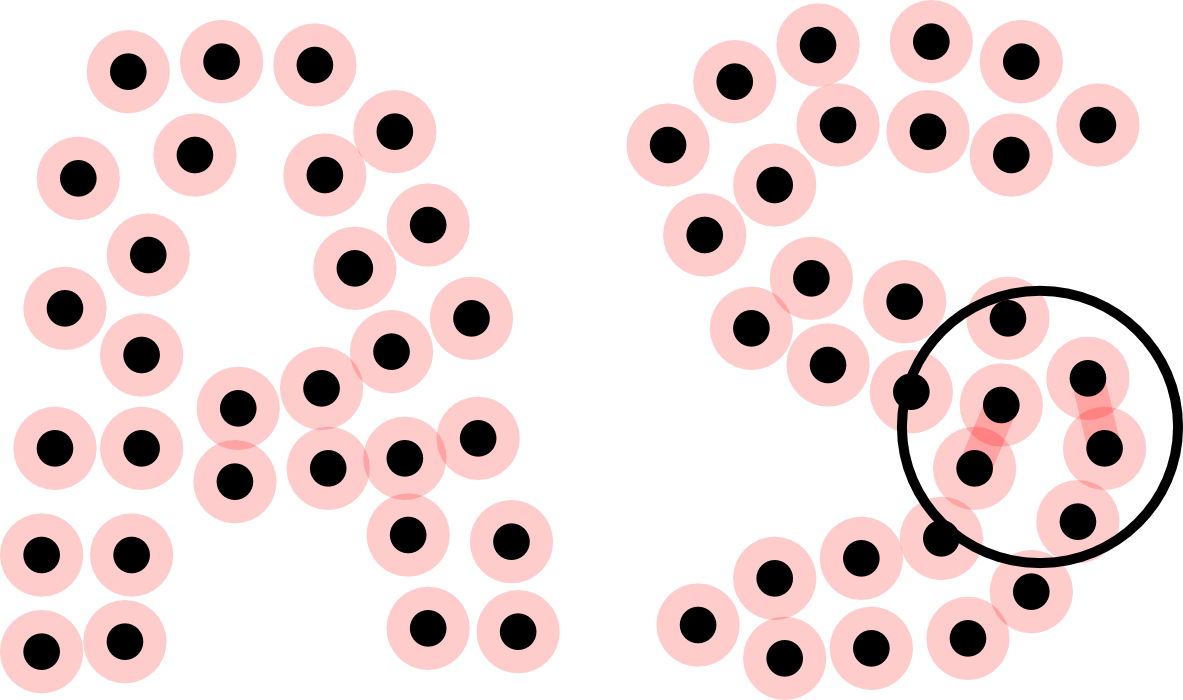
\includegraphics[scale=0.7]{../bilder/smallAS_shapeHull_closestPair.png}
	\caption{Kanten der $\alpha$-Shape verbinden dichteste Paare}
	\label{fig:shapeHull_closestPair}
\end{figure}

In Abbildung~\ref{fig:shapeHull_closestPair} ist der Bereich hervorgehoben, in welchem sich zwei dichteste Paare befinden.

Für größer werdende positive $\alpha$ existieren im Allgemeinen mehr Knoten-Paare, welche auf dem Rand einer $\alpha$-Kreisscheibe liegen. Dadurch wird die Kantenmenge größer. Die $\alpha$-Hülle entspricht derjenigen Fläche, welche nicht mehr von den $\alpha$-Kreisscheiben ausgefüllt werden kann. Punkte, welche im inneren der $\alpha$-Hülle liegen, sind nicht mehr $\alpha$-extrem und zählen damit nicht mehr zur Knotenmenge der $\alpha$-Shape.

\begin{figure}[htbp]
	\centering
	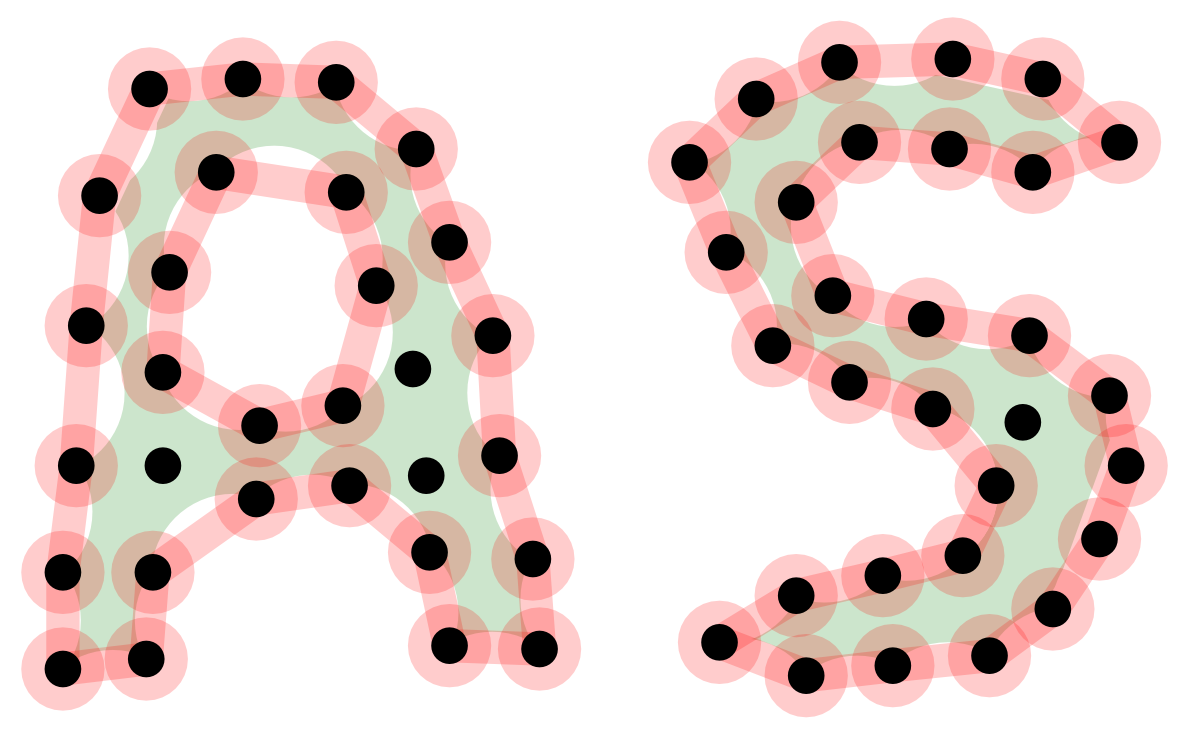
\includegraphics[scale=0.7]{../bilder/smallAS_shapeHull_positive.png}
	\caption{$\alpha$-Shape und -Hülle empfinden Gestalt sehr genau nach}
	\label{fig:shapeHull_positive}
\end{figure}

Abbildung~\ref{fig:shapeHull_positive} zeigt eine durch $\alpha$-Shape und $\alpha$-Hülle sehr genau nachempfundene Gestalt einer Punktmenge.

Variiert man $\alpha$ hin zu noch größeren Werten, so ergibt sich eine zusammenhängende $\alpha$-Shape. Einzelne Figuren werden nun durch die $\alpha$-Shape verbunden.

\begin{figure}[htbp]
	\centering
	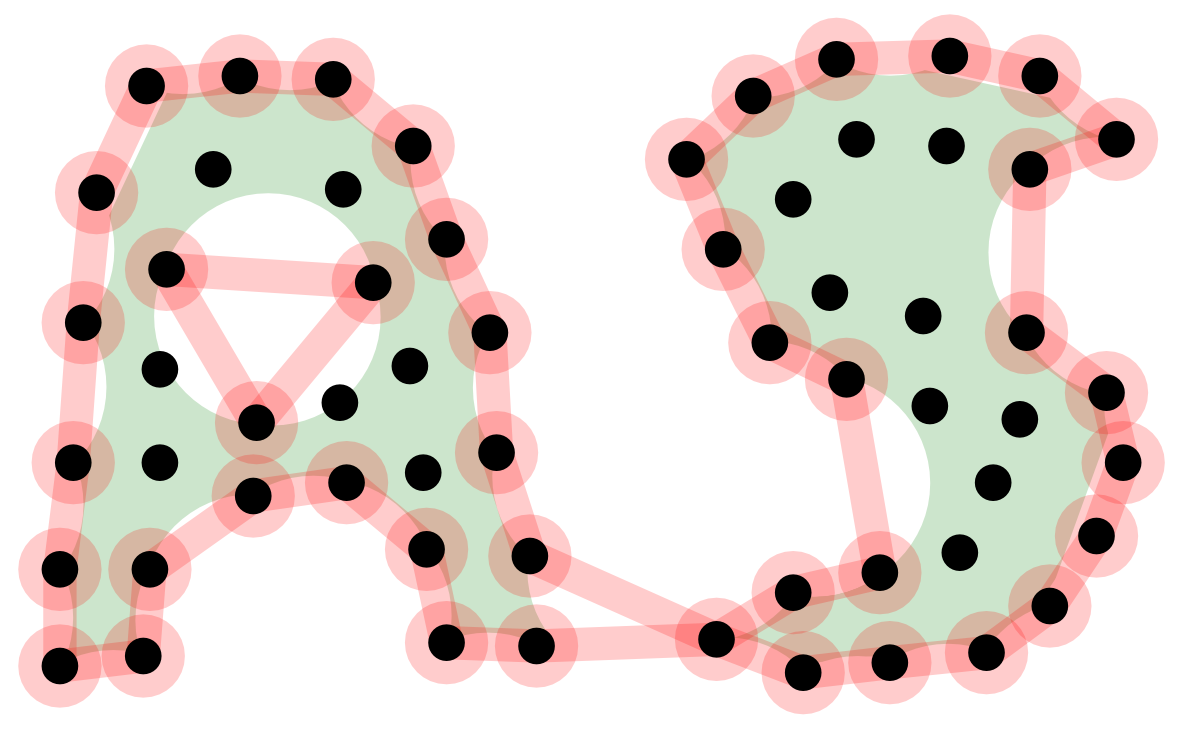
\includegraphics[scale=0.7]{../bilder/smallAS_shapeHull_connectedGraph.png}
	\caption{$\alpha$-Shape als zusammenhängender Graph}
	\label{fig:shapeHull_connectedGraph}
\end{figure}

Abbildung~\ref{fig:shapeHull_connectedGraph} zeigt eine zusammenhängende $\alpha$-Shape.

Für sehr große Werte von $\alpha$ ist nicht nur die $\alpha$-Shape ein zusammenhängender Graph, sondern auch die $\alpha$-Hülle ist eine zusammenhängende Fläche.

\begin{figure}[htbp]
	\centering
	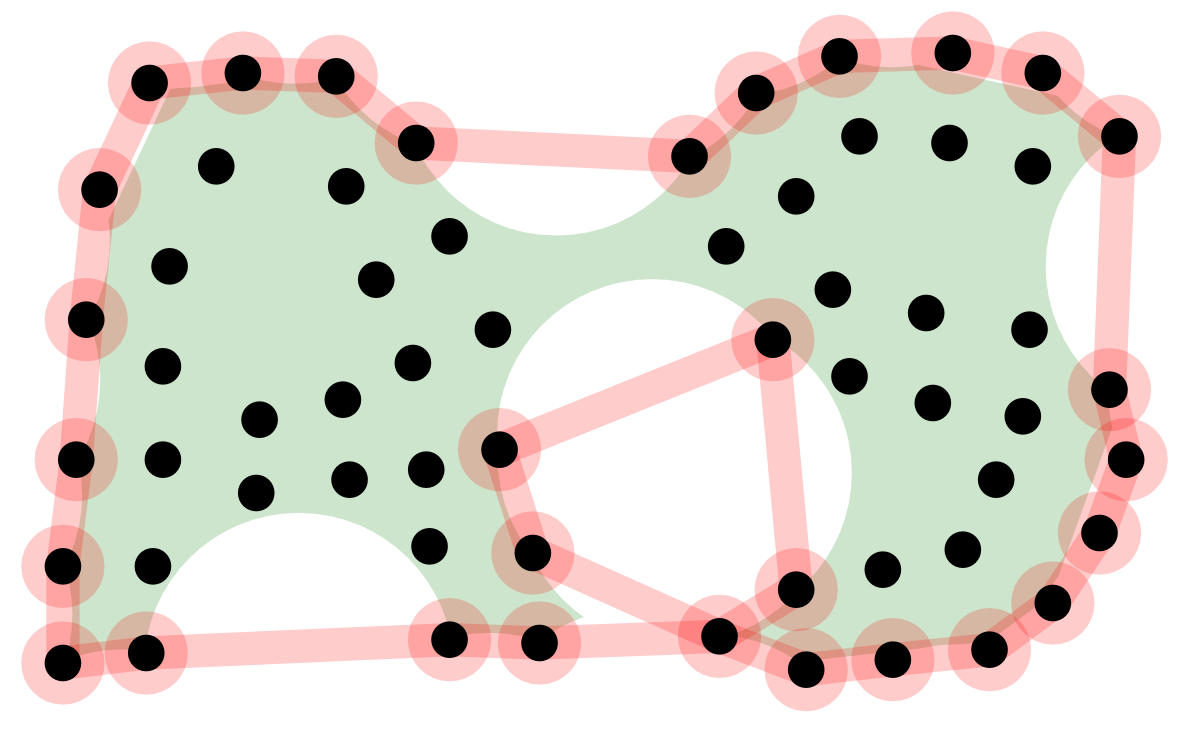
\includegraphics[scale=0.7]{../bilder/smallAS_shapeHull_connectedHull.png}
	\caption{$\alpha$-Hülle als zusammenhängende Fläche}
	\label{fig:shapeHull_connectedHull}
\end{figure}

Abbildung~\ref{fig:shapeHull_connectedHull} zeigt eine zusammenhängende $\alpha$-Hülle.

Ist $\alpha$ unendlich groß, so ist die $\alpha$-Hülle wieder gleich der konvexen Hülle.

